\chapter{Evaluation}

\section{Objective}
The study aimed to assess the usability of the current system by analysing the objective data of target posture occurrence rate in the scenario study, and the subjective data of the participants’ perspective to the system on 8 dimensions for the usability.

\section{Method}
The study included two sections. In the first section, the participants were randomly assigned into either watching TV group or using mobile device group. A Kinect would be placed in the front of where the participants sit to record the position of 25 joints in the body and a DV would videotape from the side. The participants were be asked to relax and behave like they usually did when engaging in the tested activity. Both scenarios would last for 15 minutes. Participants in the watching-TV group would watch a talk show, while the participants in the using mobile device group would be given an android phone, with the ELF installed, to use within the time. As watching TV is an activity that enables many people to engage in at the same time, the study had 2 pairs of participants to attend the scenario study together, and three participants to attend the scenario individually. On the other hand, four participants were assigned to attend the using mobile device scenario individually since it is an activity usually conducted by oneself. In summary, there would be 4 participants attending the scenario of using mobile device individually, 3 participants attending the scenario of watching TV individually, and 4 attending the scenario of watching TV individually.

The second section was an interview to investigate the perspectives of the participants to current system. Some questions were chosen from the
\textit{System Usability Scale}~\cite{sus}, as the scale was tested to have great reliability in the evaluation of a variety of applications. The other questions were generated originally to test six heuristics related to the use of current system, namely consistency and standardization, flexibility, efficiency, aesthetic and minimalist design, match between the system and the real world, and the consumption of the working memory, among the 10 usability heuristics proposed by Nielson~\cite{nielson_heuristics}. Nielson's heuristics were referenced here as they could be regarded as the principles of usability. In addition to the 6 heuristics, there were also some questions investigating the experience of receiving the feedback from each feedback functions, and a question to ask the frequency that the participants would like to use the system when they were at home. The questions were grouped to explore the 8 dimensions of usability for the system respectively.

\section{Participant}
11 university students aged between 20 and 30, body height between 155 and 173 cm (average = 165.1), with no significant musculoskeletal disorder history.

\section{Material}
\subsection{Experimental apparatus and resources}
The following materials were used to measure the posture, record the procedure, construct the system, and facilitate the interview.

\begin{itemize}
\item A Microsoft Kinect
\item A digital video
\item A projector
\item A TV display
\item A speaker
\item An android phone
\item Two computers
\item Interview statement sheet (See Appendix~\ref{appendix:interview_instructions})
\end{itemize}

\subsection{Documents for ethical concerns}
The ethical considerations of the study were approved by The University Teaching and Research Ethics Committee. The approval letter for the study could be seen in Appendix H. The following sheets were given to the participants to protect their right and ensure they understood the study.

\begin{itemize}
\item Participant Information Sheet (See Appendix~\ref{appendix:information_sheet})
\item Participant Consent Sheet (See Appendix~\ref{appendix:consent_form})
\item Participant Debriefing Form (See Appendix~\ref{appendix:debrief_form}) 
\end{itemize}

\section{Procedure}
The researcher would introduce the system as well as the objective of the study to the participant in the beginning, and ask the participant to read and sign on the consent sheet and the information sheet. The participant would be assigned into a scenario, and the scenario would begin when the participant reported he was well prepared and relax. The scenario would last for 15 minutes, with a DV videotaping from the side. After the scenario, an interview would be conducted to investigate the participant’s perspective on the usability of the system. The contents of the interview can be seen in appendix F. A briefing procedure following would enable the researcher to again explain the purpose of the study, and encourage any opinion which aroused during the study to be reported.

\section{Result and Analysis}
\subsection{Scenario Study}
In the first scenario, the participants would be asked to relax themselves and use the provided mobile device to do whatever they liked. They would receive the feedback for their postures from the android application on the mobile display and the projection system on the front wall. The participants in the scenario were detected as crossing their legs on average for 4 percent (standard deviation = 2.73) of the time, slouching for 15.3 percent (standard deviation = 6.67) of the time, and having a low viewing height for 28 percent (standard deviation = 47) of the time. The standard deviation for having a low viewing height posture was high because one participant had the posture for 98.5 of the time while the others had the posture for approximately 5 percent of the time only. Figure~\ref{fig:scenario_mobile} shows the comparisons of the target posture occurrence rate before and after the current system was applied. The occurrence rate of crossing legs decreased by 90 percent, while slouch and low viewing height also decreased by 38.9 and 35.6 percent respectively.

\begin{figure}[h]
\centering
  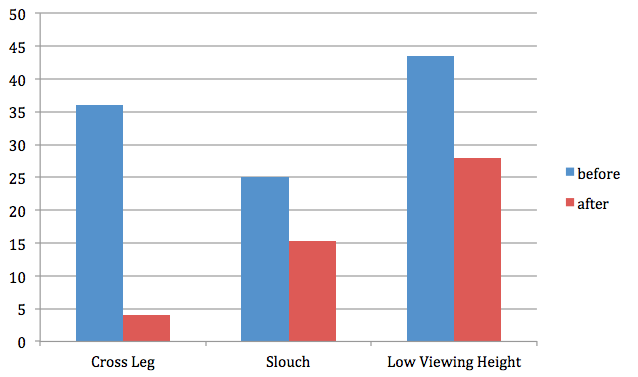
\includegraphics[width=0.5\textwidth]{figs/scenario1}
\caption{Posture occurrence rate comparison before and after the use of system in mobile device scenario}
\label{fig:scenario_mobile}
\end{figure}

In the second scenario, the participants would watch a talk show on TV and receive the feedback for their postures from the projection system on the front wall. The participants were either doing the activity by themselves or being paired with one friend. In the former condition, the participants were detected as crossing their legs on average for 12.84 percent (standard deviation = 17.1) of the time and slouching for 30.5 percent (standard deviation = 12.23) of the time. In the later condition, the participants were detected as crossing their legs for 24.5 percent (standard deviation = 4.91) of the time and slouching for 54.38 percent (standard deviation = 11.12 percent) of the time. Figure~\ref{fig:scenario_tv} shows the comparisons of the target posture posture occurrence rate before and after the current system was applied. For the participants watching TV individually, the occurrence rate of cross-leg posture decreased by 63 percent, and slouch posture decreased by 59.2. For those watching TV with another participant, the occurrence rate of cross-leg posture decreased by 29.4 percent and slouch posture decreased by 27.3 percent on average. 

\begin{figure}[h]
\centering
  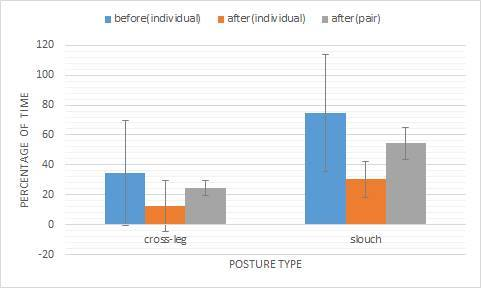
\includegraphics[width=0.5\textwidth]{figs/scenario2}
\caption{Posture occurrence rate comparison before and after the use of system in TV scenario}
\label{fig:scenario_tv}
\end{figure}

The deviation of the posture behaviour occurrence rate was caused by the small amount of participants in the study and the diversity of posture behaviour between people. The deviation of the posture behaviour in the evaluation study, however, was less than the deviation of the posture behaviour measured in the prior user study. This might also indicate that the system had some effect on the posture improvement therefore the diversity of posture behaviour pattern between the participants decreased. The procedure for the participants to change their posture behaviour pattern could be explained using the Yale attitude model. According to the Yale model, the participants should first \textit{pay attention} on the feedback, then \textit{comprehend} the content, and \textit{accept or agree} with the information. The information should be also \textit{retained} in their mind until they \textit{take action}~\cite{communication_persuasion}.

To sum up, the system improved all target posture in every scenario basically, which meant the system achieved its aim possibly using the Yale attitude model. The system had the best effect on improving cross-legs posture (90 percent in using mobile scenario and 63 percent in watching TV individually scenario) among all target bad postures. Also, the system had better effect on improving target postures when there was only one user in the environment than two users. It might because that the interaction among the users could cost their cognitive resource and reduce the possibility for the feedback in Yale model to go from one stage to another, such as the information of the feedback might stick in the stage of acceptance without continuing and enter the stage of retaining. The candidate solution for the problem would be discussed in next chapter.

\subsection{Interview}
The interview focused on eight dimensions of the system. Each dimension was assessed by the participants’ rating for one to five statements. The list of statements can be seen in Appendix F. The index of the dimension and its corresponding statements are presented in Table~\ref{tab:nonlin}. The scores of the reverse statements would be calculated backwards, and the average and standard deviation scores of each dimension would be examined. The result is presented in Figure~\ref{fig:usability_ratings}.

\begin{table}[ht]
\centering
\begin{tabular}{l c c}
Dimension&Statment Amount&Statement Nimber\\
\hline
Consistency and standardisation&2&1,2\\
Recognition rather than recall&1&4\\
Match between the system and real world&1&3\\ 
Flexibility&1&8\\
Efficiency&5&5,6,7,9,10\\ 
Aesthetic and minimalist design&2&11,12 \\
User experience&3&13,14,15\\
Frequency of use&1&16\\
[1ex]
\hline
\end{tabular}
\caption{Index of Usability Dimensions and Corresponding Statements}
\label{tab:nonlin}
\end{table}

\begin{figure}[h]
\centering
  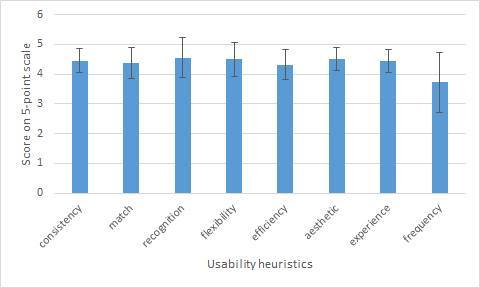
\includegraphics[width=0.5\textwidth]{figs/usability_evaluation}
\caption{Average ratings for each usability dimension on 5-point scale}
\label{fig:usability_ratings}
\end{figure}

The ratings between the participants were consistent in most statements. The average standard deviation of ratings for one statement was not higher than 0.7 in every dimension excluding the frequency of use. This is because some of the participants reported that they might not always want to improve their postures; sometimes they just wanted to relax in a comfortable posture and pay no consideration about whether it is a healthy posture or not. With the comparative high deviation, the average rating for the predicted frequency of use was also the lowest one among the all. The average 3.73 indicates the frequency for the participants to user the system would locate between sometimes and often. The other dimensions, on the other hand, were given high identification in general. The evaluation of the feedback system could also verify the posture model by including the statement of \textit{the system could catch my posture sensitively} and \textit{the system could categorise my posture correctly} in the efficiency dimension. The two statements were rated for an average 4.09 and 4.0 respectively.

The open-ended questions following investigated the perspectives of the participants to the three feedback functions respectively. The analysis was made by the interpretation of notes taken in the procedure of the interview.

\begin{enumerate}
\item Angel and Devil Clock feedback \hfill \\
The participants reported that they felt the design of the system was novel and special, and wanted to be classified into the party of angel. However, they mentioned that the system could catch their attention due to its attractive design, but also could distract their attention sometimes particularly when the label flashes when a user was firstly classified as having a good or bad posture. Also, the flowers and the bomb were respectively used as the tokens of the accumulated good posture lasting time and bad posture lasting time, but the flowers would wither due to the increase of accumulated bad posture lasting time, while the bombs would just disappear subsequently when the good posture lasting time increased. Namely, the tokens for the good posture behaviour, flower, has two types, but the tokens for the bad posture behaviour, bomb, only has one. The imbalance might confuse the users.
\item Individual Head Tracking feedback \hfill \\
Some participants felt a little bit creepy when the eyes in the face firstly show. After that, they felt the effect of the skeleton was novel and useful when the constrained joints being highlighted. They reported that they would perceive the skeleton on the wall as the reflection of the negative part of themselves, and try to wipe it out. For the downside of the design, a participant mentioned that if the user were sitting at one side of the sofa and watching a TV located in the front of the other side, the feedback could be easily ignored because the image of the spotlight would be projected on to the position where right in front of the user as the feedback for a bad posture. As there would always exist the problem of blind point for a visual feedback, the integration of the Individual Head Tracking and some audio effect could be effective. The comparison of using the cartoon-style skeleton and the user’s real skeleton image (the picture of Kinect Body Basics would be introduced) was also investigated. About 2/3 of the participants preferred the cartoon-style skeleton, because it would be less scary, and would not cost that much attention to look at compared to the amount that would be cost in their imagination. The other 1/3 said using the skeleton of the user himself would be cooler and further increase the user’s sense of involvement on the promoted issue.
\item ELF \hfill \\
Generally the participants were satisfied with the application, as it could serve in the background, easily be modified, and interact with the user by providing personalized encouragement to the user’s selected emoji. One participant suggested the system to include more emojis and increase the possible interactive methods between the user and the system, which could be a great progress for the future work. However, the analysis of the data show a drawback of using the mobile device to provide the posture feedback: the participant who behaved as most being fascinated by the application was examined as having a low viewing height posture for 98.5 percent of the time when the participant was immersed in the using mobile device activity and tried hard to explore the different functions provided by the application. Using the feedback delivered by a mobile device, which would possibly be viewed with a low viewing height posture as well, to improve the low viewing height posture could be really challenging. Other feedback form, such as an audio effect, could be integrated with the functions provided by ELF, so that the user could no longer tend to check a feedback for a low viewing height posture with a low viewing height posture. However, other media could still have better effect and be more appropriate for the improvement of low viewing height posture.
\end{enumerate}

The analysis in this chapter mainly focused on the findings from the evaluation study. More considerations and limitations about the system will be discussed in the next chapter.
